\documentclass[en]{../../../../../../eplexam}

\usepackage{wrapfig}
\usepackage[american,siunitx]{circuitikzgit} %version personelle du package circuitikz avec le modèle du cspst corrigé 
\usepackage{enumitem}

\hypertitle{elec-FSAB1201}{1}{EPL}{1201}{2016}{Août}{All}
{Nathan Jacques \and Arthur van Stratum}
{Jean-Didier Legat}

\paragraph{Question 1}
\begin{wrapfigure}[3]{l}{4cm}
	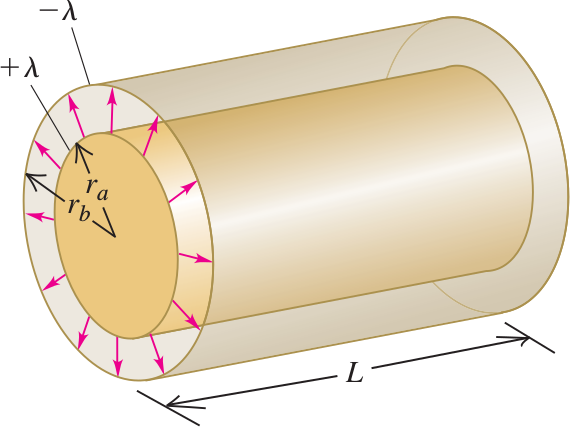
\includegraphics[width=4cm]{capa}
\end{wrapfigure}
Pour cette capacité cylindrique, on demande d'exprimer C en fonction des paramètres géométriques. Expliquer avec soin et précision votre raisonnement.
\begin{figure}
	%image
\end{figure}

\vspace{3cm}

\paragraph*{Solution}

Nous savons que \[ Q \stackrel{\Delta}{=} CV\]

Pour trouver la valeur de la capacité, il nous manque donc la différence de potentiel entre ses deux parois. Or, celle-ci peut être calculée grâce au champ électrique présent entre elles.

L'expression du champ électrique varie en fonction de $r$. Néanmoins, seul le champ entre ces deux parois (i.e. pour $r_a<r<r_b$) nous intéresse.

Pour cela, rappelons la loi de Gauss disant: $\displaystyle{\oint \vec{E} \cdot \vec{\mathrm dA} = \frac{Q_{encl}}{\epsilon_0}}$. Comme le problème est symétrique et que le champ est uniforme, cette intégrale devient triviale et il apparait que $\displaystyle{ E 2\pi rL = \frac{\lambda L}{\epsilon_0}}$ pour une surface de Gauss cylindrique de rayon $r$ et de longueur $L$. En isolant $E$, on obtient: \[E(r) = \frac{\lambda}{2\pi r \epsilon_0}\]

Calculons maintenant la différence de potentiel en sachant que $\displaystyle{V_a -V_b \stackrel{\Delta}{=} \int_a^b \vec{E}\cdot \vec{\mathrm dl}}$
\[V = \int_{r_a}^{r_b} \frac{\lambda}{2\pi r \epsilon_0} \mathrm dr = \frac{\lambda}{2\pi \epsilon_0} \int_{r_a}^{r_b} \frac{\mathrm dr}{r} = \frac{\lambda}{2\pi \epsilon_0} \ln \frac{r_b}{r_a}\]

Il vient donc
\[ \boxed{C \stackrel{\Delta}{=} \frac{Q}{V} = \frac{\lambda L}{\frac{\lambda}{2\pi \epsilon_0} \ln \left(\frac{r_b}{r_a}\right)} = \frac{2 \pi \epsilon_0 L}{\ln \left(\frac{r_b}{r_a}\right)}}\]

\paragraph{Question 2}
\begin{enumerate}[label=\alph*.]
	\item Calculez la tension $V_1$ et $V_2$;
	\item Calculez la puissance dissipée par la source de tension;
	\item Calculez la puissance dissipée par les 2 sources de courant;
	\item Calculez la puissance dissipée par toutes les résistances.
\end{enumerate}
\begin{circuitikz}%[american voltages,american currents]
	\draw 	 
		(0,0) node  (V2) {$\bullet$} to[R,l_=$10 \mathrm k\Omega$]++(4,0) node (V1) {$\bullet$} to[R=$2 \mathrm k\Omega$]++(0,-2.5) -- ++(-5.5,0) to[american current source=10mA] ++(0,2.5) --++(1.5,0)
		(V2) to[R=$2{,}5 \mathrm k\Omega$]++(0,-2.5)
		(4,0) -- ++(0,1.5) to[american current source=15mA] ++ (-4,0) -- ++(0,-1.5)
		%(4,-2.5) -- ++(3,0) to[american voltage source=10V]++(0,2.5) to [R=$1\mathrm k\Omega$](V1)
		(V1) to [R=$1\mathrm k\Omega$]++(3,0)to[american voltage source=10V]++(0,-2.5) -- (4,-2.5) node[ground]{}
		(V1) node [above right]{$V_1$}
		(V2) node [above left]{$V_2$}
	;
\end{circuitikz}


\paragraph*{Solution}

\begin{enumerate}[label=\alph*.]
	\item Nous utiliserons la méthode des noeuds aux noeuds de tensions $V_1$ et $V_2$ en supposant les courants sortant du noeud dans chaque branche (certains courants seront donc négatifs, cette méthode aide à ne pas faire d'erreurs de signe).

		Au noeud de tension $V_1$, nous établissons 
		\begin{align}
			\frac{V_1}{2\times 10^{3}} + \frac{V_1 -10}{1000} + 15 \times 10^{-3} + \frac{V_1-V_2}{10\times 10^{3}} & = & 0 \nonumber \\
			16V_1 - V_2 & = & -50
			\label{eq1}
		\end{align} 

		Au noeud de tension $V_2$, nous établissons 
		\begin{align}
			-10\times 10^{-3} -15\times 10^{-3} + \frac{V_2}{2.5\times 10^{3}} + \frac{V_2-V_1}{10\times 10^{3}} & = & 0 \nonumber \\
			5V_2-V_1 & = & 250
			\label{eq2}
		\end{align}


		En résolvant le système composé de \ref{eq1} et \ref{eq2}, on trouve aisément

		\[
			\left\{\begin{array}{l}
				V_1 = 0\mathrm V \\ V_2 = 50\mathrm V
			\end{array}\right. 
		\]

	\item Rappel: $P \stackrel{\Delta}{=} VI$

		Le courant parcourant la résistance de $1 \mathrm k\Omega$ est le même pour la source de tension. Il vaut $I = \frac{10}{1000} = 10 \mathrm{mA}$ de droite vers la gauche, la source de tension \textbf{fournit} donc $P = 10 \times I = \boxed{100 \mathrm{mW}}$
	\item Pour la source de $10 \mathrm{mA}$, $P = 0.01 \times -50 = - 500 \mathrm{mW}$. Cette source \textbf{fournit} donc $500 \mathrm{mW}$. Pour la source de $15 \mathrm{mA}$, $P = 0.015 \times -50 = -750 \mathrm{mW}$. Cette source \textbf{fournit} donc $\boxed{750 \mathrm{mW}}$
	\item Comme la tension aux bornes de la résistance de $2 \mathrm k\Omega$ est nulle, aucun courant ne la traverse et elle ne dissipe aucune puissance. Pour les autres en appliquant simplement une autre forme de la formule $P = VI = \frac{V^2}{R}$, on arrive aisément aux résultats suivants:

		\[
			\left\{\begin{array}{l}
				P_{2.5 \mathrm k\Omega} = 1\mathrm W \\ P_{10 \mathrm k\Omega} = 250\mathrm{mW} \\ P_{1 \mathrm k\Omega} = 100\mathrm{mW}
			\end{array}\right. 
		\]

		Il est évident que les résistances \textbf{dissipent} de l'énergie. Pour vérifier nos calculs, nous pouvons faire la somme des puissances ainsi trouvées qui est bel et bien nulle (conservation de l'énergie).
\end{enumerate}


\newpage

\paragraph{Question 3}
Calculez pour le circuit suivant
\begin{figure}[h]	
	\begin{circuitikz}
		\draw
		(0,2) to[american voltage source,v_=10V](0,0)
		(0,2)to [R=$4k\Omega$]++(2,0)to [R=$12k\Omega$]++(0,-2)to(0,0)
		(2,2) -- ++(2.5,0) node  (A) {$\bullet$} to[C=100nF,v_=$V_c$,i=$I_c$]++(0,-2) --++(-2.5,0)
		(4.5,2) -- ++(2,0)to[R=$4k\Omega$]++(0,-2) --++(-2,0)
		(6.5,2)to [R=$12k\Omega$]++(2,0)to [american voltage source,v^=10V]++(0,-2)--++(-2,0)
		(4.5,2)--++(0,1.5) to[cspst,l=t{=}0]++(6,0) to[R=$1.5k\Omega$]++(0,-3.5)--++(-2,0)
		;
	\end{circuitikz}
\end{figure}
\begin{enumerate}[label=\alph*.]
	\item la tension $V_c(t)$ pour $t < 0$;
	\item la tension $V_c(t)$ pour $t \geq 0$; 
	\item le courant $I_c(t)$ pour $t \geq 0$; 
	\item le circuit équivalent de Thévenin par C pour $t \geq 0$.
\end{enumerate}

\vspace{2cm}

\paragraph*{Solution}

\begin{enumerate}[label=\alph*.]
	\item En $t < 0$, l'interrupteur est ouvert, la branche de droite est déconnectée et nous nous en passons pour l'analyse du circuit. De plus, le circuit est en régime stable, ce qui signifie qu'une certaine charge se trouve aux bornes du condensateur et il peut donc être cpnsidéré comme un circuit ouvert. Ce qui nous laisse

		\begin{figure}[h!]
			\begin{center}
				\begin{circuitikz}

					\draw 
					(0,2) to[V, l_=\mbox{$\SI{10}{\volt}$}](0,0)
					(0,2) to[R=$4\mathrm k\Omega$,-*](2,2) node[label={above:A}] {}
					(2,2) to[R=$3\mathrm k\Omega$,v=$V_c$,*-](2,0) node[ground] {} (2,-1)
					(2,0) to[short](0,0);
					\draw
					(2,2) to[R=$12\mathrm k\Omega$,*-](4,2)
					(4,2) to[voltage source,v=10V](4,0)
					(4,0) to[short](2,0);

				\end{circuitikz}
			\end{center}
		\end{figure}

		En appliquant la méthode des n\oe uds au n\oe ud A, on trouve facilement
		\begin{align*}
			\frac{V_c-10}{4\mathrm k}+\frac{V_c}{3\mathrm k}+\frac{V_c-10}{12\mathrm k} & = & 0 \\
			3V_c-30+4V_c+V_c-10 & = & 0\\
			V_c(t<0) & = & 5\mathrm V
		\end{align*}

	\item Pour trouver l'expression de $V_c(t)$, calculons $V_c(t=\infty)$. Maintenant, l'interrupteur est fermé et la résistance de 5k se retrouve en parallèle avec le condensateur. A nouveau, le circuit est en steady-state. Ce qui nous laisse

		\begin{figure}[h!]
			\begin{center}
				\begin{circuitikz}

					\draw 
					(0,2) to[V, l_=\mbox{$\SI{10}{\volt}$}](0,0)
					(0,2) to[R=$4\mathrm k\Omega$,-*](2,2) node[label={above:A}] {}
					(2,2) to[R=$1\mathrm k\Omega$,v=$V_c$,*-](2,0) node[ground] {} (2,-1)
					(2,0) to[short](0,0);
					\draw
					(2,2) to[R=$12\mathrm k\Omega$,*-](4,2)
					(4,2) to[voltage source,v=10V](4,0)
					(4,0) to[short](2,0);

				\end{circuitikz}
			\end{center}
		\end{figure}

		En appliquant la méthode des n\oe uds au n\oe ud A, on obtient

		\begin{align*}
			\frac{V_c-10}{4\mathrm k}+\frac{V_c}{1\mathrm k}+\frac{V_c-10}{12\mathrm k} & = & 0\\
			V_c(t=\infty) & = & 2.5 \mathrm V
		\end{align*}

		\[V_c(t)= V_c(t=\infty) +(V_c(t<0) - V_c(t=\infty))\mathrm{e}^{\frac{-t}{\tau}} = \boxed{2.5 + 2.5 \mathrm{e}^{\frac{-t}{\tau}}\mathrm{V}}\]

		où $\tau = RC$ est la constante de temps du circuit. Pour calculer celle-ci, il nous manque la résistance équivalente du dipôle de Thévenin aux bornes du condensateur. Pour l'obtenir, il suffit de "court-circuiter" les deux sources de tension et nous nous retrouvons avec les trois résistances de 4k, 12k et 1k en parallèle, ce qui nous donne une résistance équivalente $R_{eq}=750 \Omega$.
		\[\tau = RC = 750 \Omega \times 100 \mathrm{nF} = \boxed{75 \mathrm{\mu s}}\]

	\item Nous savons que $\displaystyle{I_c = C\frac{\mathrm dV}{\mathrm dt}}$. On trouve aisément
		\[\frac{\mathrm dV}{\mathrm dt} = \frac{\mathrm d}{\mathrm dt}\left(2.5+2.5\mathrm{e}^{\frac{-t}{\tau}}\right) = 2.5\left(\frac{-1}{\tau}\right) \mathrm{e}^{\frac{-t}{\tau}}\]

On obtient donc
\[I_c(t \geq 0) = C\frac{\mathrm dV}{\mathrm dt} = 100\times 10^{-9}\times 2.5\left(\frac{-1}{\tau}\right) \mathrm{e}^{\frac{-t}{\tau}} = \boxed{\frac{-10}{3}\mathrm{e}^{\frac{-t}{\tau}} \mathrm{mA}}\]
avec $\tau = 75 \mathrm{\mu s}$

\item La tension de Thévenin est la tension de circuit-ouvert aux bornes du condensateur, que nous avons calculée ci-dessus et vaut $V_{th}= 2.5 \mathrm V$

	L'équivalent de Thévenin est donc


\begin{figure}[h!]
	\begin{center}
		\begin{circuitikz}

			\draw 
			(2,2) to[R, l_=\mbox{$R_{eq}=750\Omega$},o-](0,2)
			(0,2) to[V, l_=\mbox{$V_{th}=\SI{2.5}{\volt}$}](0,0)
			(0,0) to[short,-o](2,0)
			(2,0) to[open,v<=$V_{th}$](2,2);

		\end{circuitikz}
	\end{center}
\end{figure}


\end{enumerate}

\newpage

\paragraph{Question 4}
Soit un circuit RLC série. On vous demande (expliquer avec soin et précision votre raisonnement)
\begin{itemize}
	\item de déduire l'expression de l'impédance $Z$ et du déphasage $\phi$;
	\item de dessiner le diagramme phasoriel pour $X_L>X_C$;
	\item de déduire une expression de la puissance moyenne $P_{average}$ fournie.
\end{itemize}

\vspace{2cm}

\paragraph*{Solution}




\begin{enumerate}
	\item L'impédance $Z$ est la somme vectorielle des réactances et de la résistance du circuit. Sur le diagramme phasoriel ci-dessous, la somme de la tension aux bornes de la self et du condensateur nous donne $\displaystyle{I\left( X_L-X_C\right)}$. Additionnons le vecteur représentant la tension aux bornes de la résistance et nous obtenons, par Pythagore, $\displaystyle{V = \sqrt{I^2R^2+I^2\left( X_L-X_C\right) ^2}}$. Or, comme $\displaystyle{V =IZ}$, si on divise chaque membre par $I$
		\[\boxed{Z = \sqrt{R^2+\left( X_L-X_C\right) ^2}}\]

		Le déphasage est l'angle avec lequel le voltage $v = V_{max}\cos\left( \omega t + \phi\right) $ devance le courant $i =I_{max}\cos\left( \omega t\right) $ , il sera donc négatif si le voltage devait suivre le courant. Par les règles de trigonométrie dans le triangle rectangle, on voit que $\displaystyle{\tan{\phi} = \frac{X_L-X_C}{R}}$ et donc
		\[\boxed{\phi = \arctan \left(\frac{X_L-X_C}{R}\right) }\]

	\item Voir ci-dessous

	\item \[ p = vi = \left[V_{max}\cos\left( \omega t + \phi\right)\right] \left[ I_{max}\cos\left( \omega t\right)\right]\]
		Développons par la formule du cosinus d'une somme,
		\begin{align*}
			p & = & \left[V_{max}\left( \cos (\omega t)\cos \phi -\sin (\omega t)\sin \phi\right)\right] \left[ I_{max}\cos\left( \omega t\right)\right]\\
			& = & V_{max}I_{max} \cos \phi \cos ^2(\omega t) - V_{max}I_{max}\sin \phi \cos (\omega t)\sin (\omega t)
		\end{align*}

		Prenons maintenant la moyenne de cette expression. La moyenne de $\cos ^2 (\omega t)$ vaut $\frac{1}{2}$ (pour vous en convaincre, transformer par Carnot); $\cos (\omega t)\sin (\omega t) = \frac{1}{2} \sin (2\omega t)$ dont la moyenne vaut zéro (facile à voir sur un graphe), il nous reste donc
		\[\boxed{P_{av}=\frac{1}{2}V_{max}I_{max}\cos \phi = V_{RMS}I_{RMS}\cos \phi}\]

\end{enumerate}

\begin{figure}[h!]
	\centering
	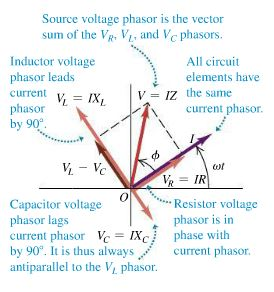
\includegraphics[scale=1]{phasors}
	\caption{$X_L > X_C$}
\end{figure}

\end{document}
